%----------------------------------------------------------------------------------------
%	PACKAGES AND OTHER DOCUMENT CONFIGURATIONS
%----------------------------------------------------------------------------------------

\documentclass[twoside,twocolumn]{article}

\usepackage{blindtext} % Package to generate dummy text throughout this template 
\usepackage{graphicx}
\usepackage{hyperref}
\usepackage{amsmath}

%% \usepackage[sc]{mathpazo} % Use the Palatino font
\usepackage[T1]{fontenc} % Use 8-bit encoding that has 256 glyphs
\linespread{1.05} % Line spacing - Palatino needs more space between lines
\usepackage{microtype} % Slightly tweak font spacing for aesthetics

\usepackage[english]{babel} % Language hyphenation and typographical rules

%% \usepackage[hmarginratio=1:1,top=32mm,columnsep=20pt]{geometry} % Document margins
\usepackage[hmarginratio=1:1,top=60pt,columnsep=20pt,left=60pt, right=60pt]{geometry} % Document margins
\usepackage[hang, small,labelfont=bf,up,textfont=it,up]{caption} % Custom captions under/above floats in tables or figures
\usepackage{booktabs} % Horizontal rules in tables

%% \usepackage{lettrine} % The lettrine is the first enlarged letter at the beginning of the text

%% \usepackage{enumitem} % Customized lists
%% \setlist[itemize]{noitemsep} % Make itemize lists more compact

\usepackage{abstract} % Allows abstract customization
\renewcommand{\abstractnamefont}{\normalfont\bfseries} % Set the "Abstract" text to bold
%% \renewcommand{\abstracttextfont}{\normalfont\small\itshape} % Set the abstract itself to small italic text

\usepackage{titlesec} % Allows customization of titles
\renewcommand\thesection{\roman{section}} % Roman numerals for the sections
\renewcommand\thesubsection{\roman{section}.\roman{subsection}} % roman numerals for subsections
%% \titleformat{\section}[block]{\large\scshape\centering}{\thesection.}{1em}{} % Change the look of the section titles
\titleformat{\section}[block]{\large\scshape\centering\bfseries}{\thesection.}{1em}{} % Change the look of the section titles
\titleformat{\subsection}[block]{\normalsize\scshape\centering}{\thesubsection.}{1em}{} % Change the look of the section titles

\usepackage{fancyhdr} % Headers and footers
\pagestyle{fancy} % All pages have headers and footers
\fancyhead{} % Blank out the default header
\fancyfoot{} % Blank out the default footer
\fancyhead[C]{MIT JLab: Detect GW from a Binary Black Hole Merger with LIGO open data} % Custom header text
\fancyfoot[RO,LE]{\thepage} % Custom footer text

\usepackage{titling} % Customizing the title section

\usepackage{hyperref} % For hyperlinks in the PDF

%%
%% ====================>>>>>>>>>>>>>>>>>>>>
%% Utility
%% <<<<<<<<<<<<<<<<<<<<====================
\newcommand{\doi}[1]{\textsc{doi}: \href{http://doi.org/#1}{\nolinkurl{#1}}}
\newcommand{\arxivv}[1]{\href{https://arxiv.org/abs/#1}{\nolinkurl{arXiv:#1}}}
\newcommand{\urll}[1]{\textsc{url}: \href{#1}{\nolinkurl{#1}}}
%% \makeatletter
%% \def\@cite#1#2{\textcolor{colorcite}{[#1\if@tempswa , #2\fi]}}
%% \def\@biblabel#1{\textbf{\textcolor{colorcite}{[#1]}}}
%% \makeatother

\newcommand{\colorbf}[2]{{\textbf{\textcolor{#1}{#2}}}}

\newcommand{\rmdme}[1]{\colorbf{red}{(rmdme: #1!!)}}
\newcommand{\capleft}{\textcolor{colorcap}{(Left) }}
\newcommand{\capright}{\textcolor{colorcap}{(Right) }}
\newcommand{\captop}{\textcolor{colorcap}{(Top) }}
\newcommand{\capbottom}{\textcolor{colorcap}{(Bottom) }}
\newcommand{\capmiddle}{\textcolor{colorcap}{(Middle) }}

\newcommand{\secref}[1]{Section~\textcolor{colorlink}{\ref{#1}}}
\newcommand{\figref}[1]{Figure~\textcolor{colorlink}{\ref{#1}}}
\newcommand{\tabref}[1]{Table~\textcolor{colorlink}{\ref{#1}}}
\newcommand{\eqqref}[1]{Eq.~\textcolor{colorlink}{(\ref{#1})}}

\renewcommand{\labelitemi}{$\circ$}
\newcommand{\tabincell}[2]{\begin{tabular}{@{}#1@{}}#2\end{tabular}}

%----------------------------------------------------------------------------------------
%	TITLE SECTION
%----------------------------------------------------------------------------------------

\setlength{\droptitle}{-4\baselineskip} % Move the title up
\pretitle{\begin{center}\large\bfseries} % Article title formatting
\posttitle{\end{center}} % Article title closing formatting
\title{Detect GW from a Binary Black Hole Merger with LIGO open data} % Article title
\author{\normalsize{MIT Department of Physics} \\
  \normalsize{(\today)}
}
%% \date{\normalsize{(\today)}} % Leave empty to omit a date
\date{} % Leave empty to omit a date
\renewcommand{\maketitlehookd}{%
\begin{abstract}
\noindent In 2016, The LIGO (The Laser Interferometer Gravitational-Wave Observatory) collaboration reported the first direct detection of gravitational waves from a binary black hole system merging to form a single black hole. GW detections would provide new tests of generay relativity especially in strong-field regime, and GW observations have become an important new means to learn about the Universe. In this project, you will understand how a GW event signal looks like, analyze the open data from LIGO, and find the mass and distance of the binary black hole system and other sources. 
\end{abstract}
}

%----------------------------------------------------------------------------------------

\begin{document}

% Print the title
\maketitle

%----------------------------------------------------------------------------------------
%	ARTICLE CONTENTS
%----------------------------------------------------------------------------------------

\section[Introduction]{introduction}\label{sec:intro}

The existence of gravitational waves (GW) was first predicted by Albert Einstein in his General Theory of Relativity in 1916.
He found that the linearized weak-field equations had wave solutions.
By analogy to electromagnetism, time variation of the mass quadrupole moment of the source is expected to lead to transverse waves of spatial strain.
The existence of GW was first demonstrated in 1974 by the discovery of a binary system composed of a pulsar in orbit around a neutron star by Hulse and Taylor~\cite{1975ApJ...195L..51H}.
\begin{figure}[hbpt]
  \begin{center}
    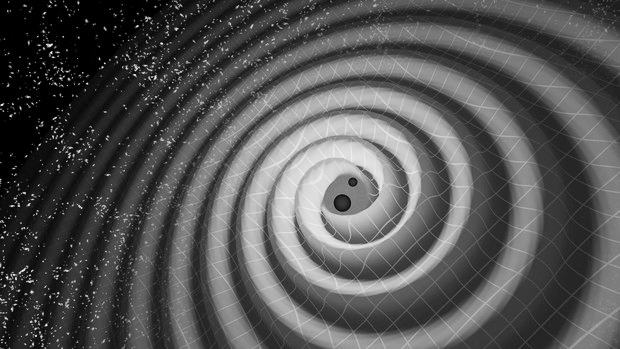
\includegraphics[width=0.48\textwidth]{figure/Gravity_Waves_StillImage_BW.png}
  \end{center}
  \caption{Illustration showing the merger of two black holes and the gravitational waves that ripple outward as the black holes spiral toward each other. \href{https://www.ligo.caltech.edu/image/ligo20160615f}{Image credit: LIGO/T. Pyle.}}
  \label{fig:intro.illustrate}
\end{figure}
However, direct detections of GW did not arrive until 2016.
In that year, The LIGO (The Laser Interferometer Gravitational-Wave Observatory) collaboration reported the first direct detection of GW from a binary black hole system merging to form a single black hole~\cite{PhysRevLett.116.061102}. 
The observations reported in this paper and futher GW detections would provide new tests of generay relativity in its strong-field regime, and GW observations have become an important new means to learn about the Universe.

In this project, you will reproduce the results reported in \cite{PhysRevLett.116.061102} with LIGO open data\footnote{\url{https://www.gw-openscience.org/about/}}. A tutorial has been prepared\footnote{\url{http://web.mit.edu/jwang011/www/LIGOtutorialJLab.html}} to show how to analyze a particular GW event GW150914. In the tutorial, you will find how to download the data collected by LIGO starting from Mon Sep 14 09:16:37 GMT 2015, plot the strain, whiten and filter the strain, plot a q-transform of the data, and extract the features of the source with a simple analytic model. After getting familiar with the basic analysis method, you need to explore more events, check the consistence between detectors, match numerical relativity waveform template to extract accurate information of the source, compare with LIGO published results, and develop a machinery to search GW event within a long time range.

%------------------------------------------------

\section[LIGO detector]{ligo detector\footnote{This section quotes the description in Ref.~\cite{PhysRevLett.116.061102}.}}\label{sec:detector}
LIGO operates two gravitational wave observatories in unison: the LIGO Livingston Observatory in Livingston, Louisiana, and the LIGO Hanford Observatory, on the DOE Hanford Site, located near Richland, Washington. These sites each operate a single Advanced LIGO detector~\cite{2015AdvancedLIGO}, a modified Michelson interferometer (see Figure~\ref{fig:detector.interf}) that measures GW strain as a difference in length of its orthogonal arms.
\begin{figure}[hbpt]
  \begin{center}
    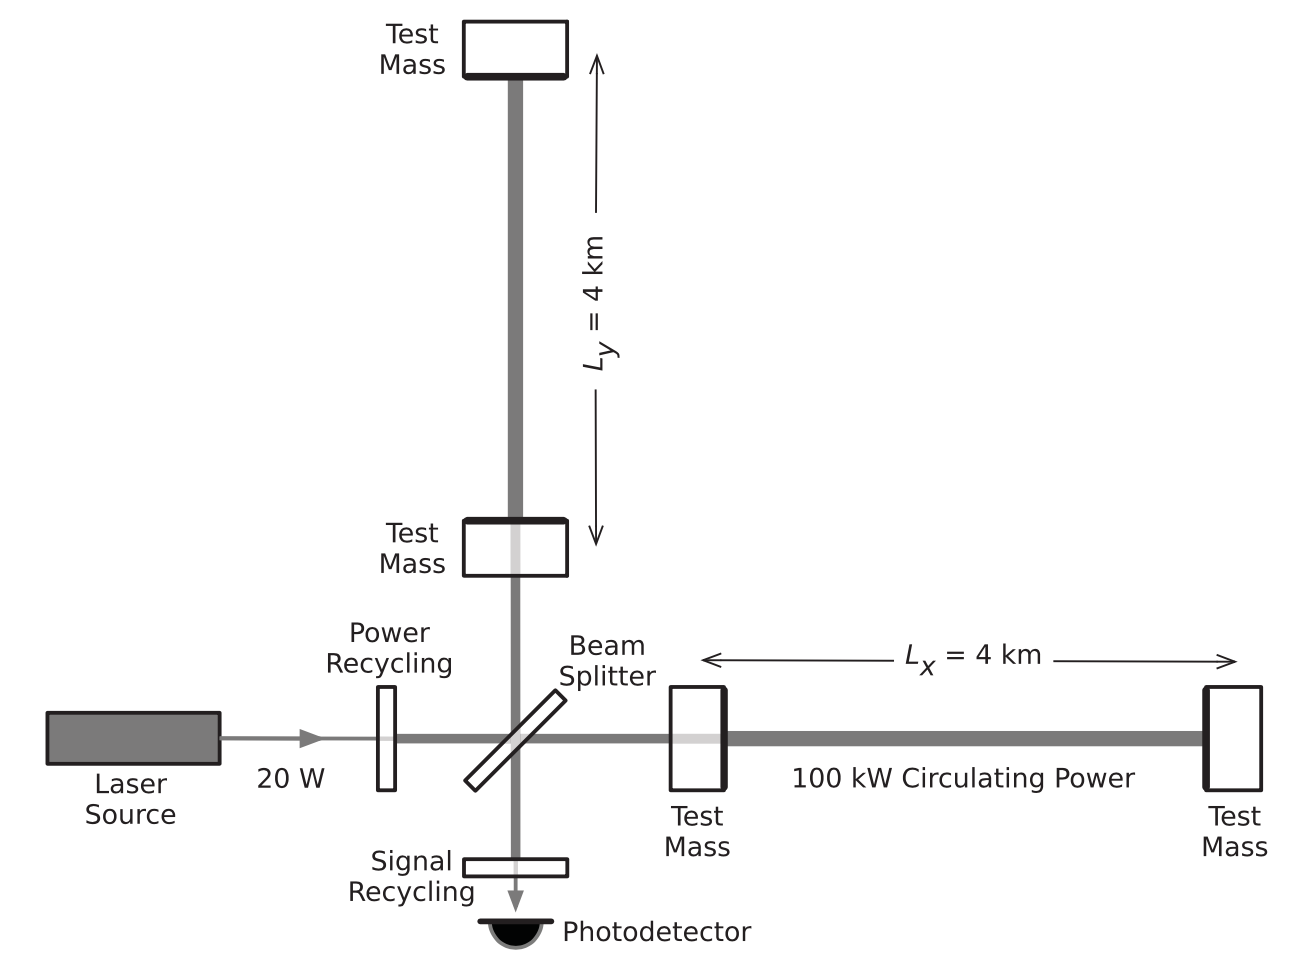
\includegraphics[width=0.48\textwidth]{figure/interference.png}
  \end{center}
  \caption{Simplified diagram of an Advanced LIGO detector (not to scale). Figure from ~\cite{PhysRevLett.116.061102}.}
  \label{fig:detector.interf}
\end{figure}
Each arm is formed by two mirrors, acting as test masses, separated by $L_{x} = L_{y} = L = 4~\mathrm{km}$. A passing GW effectively alters the arm lengths such that the measured difference is $\Delta L(t) = \delta L_{x}-\delta L_{y} = h(t)L$, where $h$ is the gravitational-wave strain amplitude projected onto the detector. This differential length variation alters the phase difference between the two light fields returning to the beam splitter, transmitting an optical signal proportional to the gravitational-wave strain to the output photodetector.

%------------------------------------------------

\section[Observation]{observation}\label{sec:observation}
The signal GW150914 detected by LIGO Hanford observatory is shown in Figure~\ref{fig:obs.h1}. 
\begin{figure}[hbpt]
  \begin{center}
    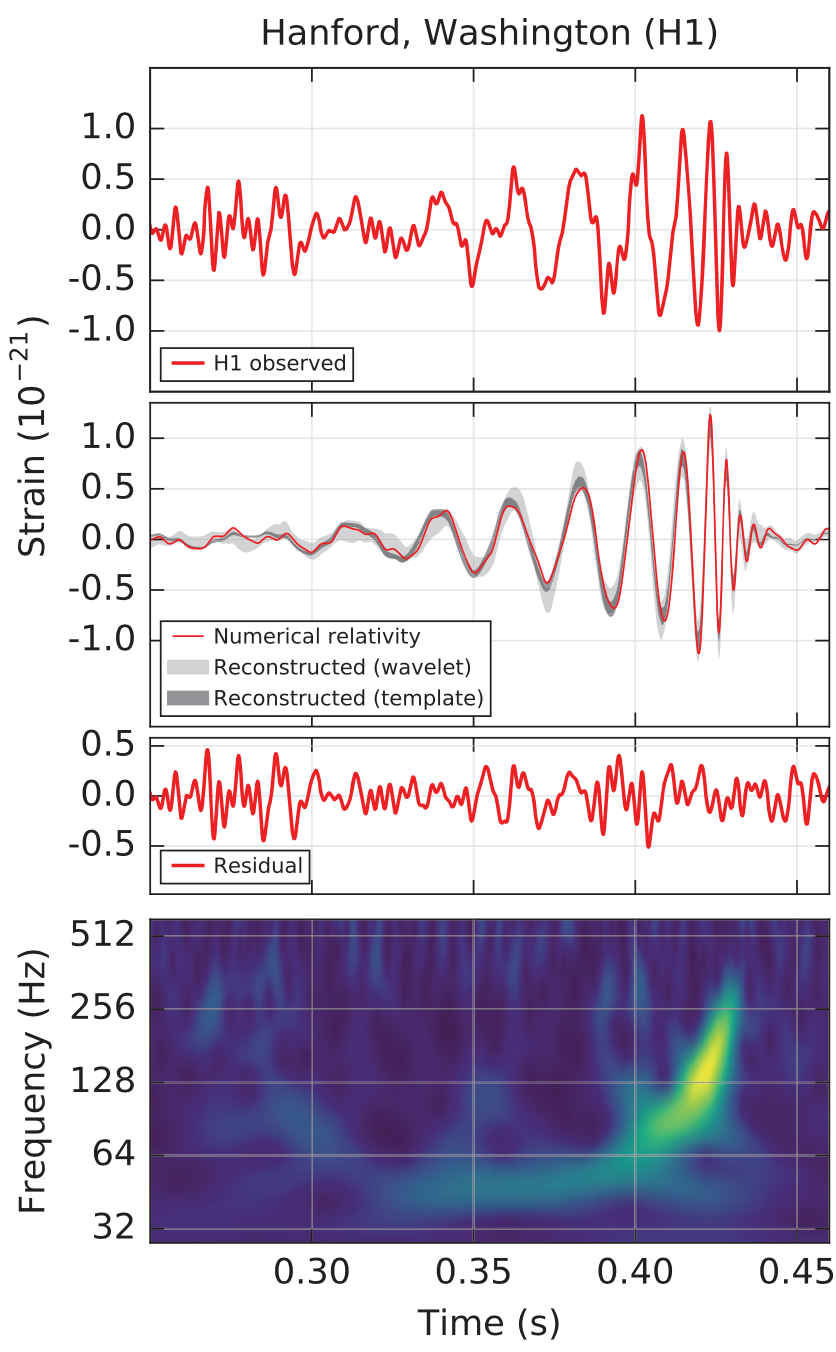
\includegraphics[width=0.48\textwidth]{figure/signalH1.png}
  \end{center}
  \caption{The gravitational-wave event GW150914 observed by the LIGO Hanford detectors. \textbf{Top row:} H1 strain data. \textbf{Second row:} Gravitational-wave strain projected onto H1 in the 35--350 Hz band. Solid lines show a numerical relativity waveform for a system with parameters consistent with those recovered from GW150914. \textbf{Third row:} Residuals after subtracting the filtered numerical relativity waveform from the filtered detector time series. \textbf{Bottom row:} A time-frequency representation of the strain data, showing the signal frequency increasing over time.}
  \label{fig:obs.h1}
\end{figure}
This event features (very likely) two inspiraling black holes merging into a single black hole (ring-down). The top raw of Figure~\ref{fig:obs.h1} shows the strain. At first, the wave shape shows the characteristics of a compact inspiral binary system. As the two objects get close, the amplitude and frequency increases. The amplitude reaches the maximum while the two objects are merging. Finally, after ringdown happens, the wave shape vanishes.

%------------------------------------------------

\section[Simple analytic calculation]{simple analytic calculation}\label{sec:analytic}
Calculating the actual waveform requires complicated numerical simulations, as shown by the second row of Figure~\ref{fig:obs.h1}. However, we can use the basic knowledge of General Relativity (GR) and Newtonian mechanics to perform an approximate analytic calculation for the waveform. For an orbiting binary system ($m_{1}$ and $m_{2}$), according to GR the frequency ($\omega$) of the GW radiation satisfies
\begin{equation}\label{eq:wwdot}
  \dot{\omega} = \frac{12}{5}2^{\frac{1}{3}}\left(\frac{G\mathcal{M}_{c}}{c^{3}}\right)^{\frac{5}{3}}\omega^{\frac{11}{3}}
\end{equation}
where $G$ and $c$ are gravitational constant and the speed of light respectively. $\mathcal{M}_{c}$ is so-called chirp mass~\cite{PhysRevLett.74.3515}, defined by
\begin{equation}\label{eq:Mc}
  \mathcal{M}_{c} = \frac{(m_{1}m_{2})^{\frac{3}{5}}}{(m_{1}+{m_{2}})^{\frac{1}{5}}}
\end{equation}
Integrating Eq.~\eqref{eq:wwdot}, we can get
\begin{equation}\label{eq:wt}
  \begin{split}
    \int\omega^{-\frac{11}{3}}d\omega &= \int\frac{12}{5}2^{\frac{1}{3}}\left(\frac{G\mathcal{M}_{c}}{c^{3}}\right)^{\frac{5}{3}}dt \\
    \Rightarrow \omega(t) &= \frac{5^{\frac{3}{8}}}{4}\left(\frac{c^{3}}{G\mathcal{M}_{c}}\right)^{\frac{5}{8}}\Delta t^{-\frac{3}{8}} \\
  \end{split}
\end{equation}
Now we get the time dependence of frequency, corresponding to the bottom row of Figure~\ref{fig:obs.h1}. Considering
\begin{equation}\label{eq:msolar}
  \frac{GM_{\odot}}{c^{3}} \approx 4.93~\mathrm{\mu s}
\end{equation}
We have
\begin{equation}\label{eq:wtnum}
  \omega(t) = 948.5\left(\frac{M_{\odot}}{\mathcal{M}_{c}}\right)^{\frac{5}{8}}\left(\frac{1\:\mathrm{s}}{\Delta t}\right)^{\frac{3}{8}}\;\mathrm{[Hz\cdot rad]}
\end{equation}
which can be used to compare with the time-frequency representation of the strain data.
Next, we build the waveform with the radiation power $dE(t)/dt$.
\begin{equation}\label{eq:ft}
  \begin{split}
    f(t) &= A(t)\cos(\omega(t)\Delta t +\phi) \\
    &\propto \frac{dE(t)}{dt}\cos(\omega(t)\Delta t +\phi) \\
  \end{split}
\end{equation}
With Newtonian mechanics, we know the energy of a binary orbit is
\begin{equation}\label{eq:Etot}
  \begin{split}
    E &= E_{\mathrm{k}} + E_{\mathrm{u}} \\
    &= \frac{1}{2}\mu\dot{r}^{2} + \frac{1}{2}\frac{m_{1}m_{2}}{m_{1}+m_{2}}\omega^{2}R^{2} - \frac{Gm_{1}m_{2}}{R} \\
    &= \frac{1}{2}\frac{m_{1}m_{2}}{m_{1}+m_{2}}\omega^{2}R^{2} - \frac{Gm_{1}m_{2}}{R} \\
  \end{split}
\end{equation}
The last step is because $\dot{r} = 0$. According to Kepler's third law,
\begin{equation}\label{eq:kepler}
  \omega^{2} = \frac{G(m_{1}+m_{2})}{R^{3}}
\end{equation}
Put Eq.~\eqref{eq:kepler} into Eq.~\eqref{eq:Etot} and substitute $R$, we have
\begin{equation}\label{eq:Ew}
  \begin{split}
    E &= -\frac{Gm_{1}m_{2}}{2R} \\
    &\propto \mathcal{M}_{c}^{\frac{5}{3}}\omega(t)^{\frac{2}{3}} \\
  \end{split}
\end{equation}
Perform derivatives on Eq.~\eqref{eq:Ew},
\begin{equation}\label{eq:dEdt}
  \begin{split}
    \frac{dE}{dt} &\propto \mathcal{M}_{c}^{\frac{5}{3}}\omega(t)^{-\frac{1}{3}}\dot{\omega} \\
    &\propto \left(\mathcal{M}_{c}\omega(t)\right)^{\frac{10}{3}} \\
  \end{split}
\end{equation}
The last step used Eq.~\eqref{eq:wwdot}. Put Eq.~\eqref{eq:dEdt} into Eq.~\eqref{eq:ft}, we have the waveform
\begin{equation}\label{eq:fwt}
  \begin{split}
    f(t) &= C\left(\mathcal{M}_{c}\omega(t)\right)^{\frac{10}{3}}\cos(\omega(t)\Delta t +\phi), \\
    \mathrm{where}\:\omega(t) &= 948.5\left(\frac{M_{\odot}}{\mathcal{M}_{c}}\right)^{\frac{5}{8}}\left(\frac{1\:\mathrm{s}}{\Delta t}\right)^{\frac{3}{8}}\;\mathrm{[Hz\cdot rad]} \\
  \end{split}
\end{equation}
and $C$ is a constant. This waveform amplitude is only supposed to work before merger ($t \leq t_{0}$), and we need to come up with a way to define the ringdown amplitude ($t > t_{0}$). The actual way to get the amplitude requires months of a super computer to build good templates. As a simple approximate solution, you can use a simple damping function (e.g. exponential). In this way, this approximate waveform can be used to fit real data.

%------------------------------------------------

\section[Analysis procedure]{analysis procedure}\label{sec:analysis}
The analysis procedure is documented in the tutorial \url{http://web.mit.edu/jwang011/www/LIGOtutorialJLab.html}, and we just quickly summarize here. The tutorial shows the procedures analyzing a particular event:
\begin{itemize}
\item Download and read data;
\item Plot the raw data strain;
\item Whiten and filter data;
\item Plot a q-transform of the data and compare to the analytic model;
\item Fit the whitened and filtered strain with the analytic model, and get the chirp mass of the binary black holes.
\end{itemize}
After getting known the method, you need to explore the following topics
\begin{itemize}
\item Check and quantify the consistence between detectors (H1 and V1);
\item Develop a machinery to search signal within a long range of time;
\item Load the template database, fit the data, and get more accurate parameters;
\item Determine how far the source of GW is away;
\item Explore more events;
\item How to determine if the source is black hole merger or neutron star merger or other source?
\end{itemize}


%------------------------------------------------


%----------------------------------------------------------------------------------------
%	REFERENCE LIST
%----------------------------------------------------------------------------------------

%% \begin{thebibliography}{99} % Bibliography - this is intentionally simple in this template

%% \bibitem[Figueredo and Wolf, 2009]{Figueredo:2009dg}
%% Figueredo, A.~J. and Wolf, P. S.~A. (2009).
%% \newblock Assortative pairing and life history strategy - a cross-cultural
%%   study.
%% \newblock {\em Human Nature}, 20:317--330.
 
%% \end{thebibliography}

%----------------------------------------------------------------------------------------

%% \addcontentsline{toc}{chapter}{references}
\bibliographystyle{thisthesis}
\bibliography{LIGOmanual}

\end{document}
